\chapter{State of the art}
In the following, we will first look at BERT in order to have the basis for all further approaches that will be considered here. BERT is followed by BioBERT, the first variation of BERT that we will look at. These two approaches are two approaches underlying SciBERT, in the sense that they were developed before SciBERT. After BioBERT we will briefly look at S2ORC-BERT which targets a specific domain similar to BioBERT. Last but not least comes AOG-BERT which tries, with a more extensive modification to BERT, to convey further information which otherwise are not explicitly considered in the BERT model. After these approaches we will turn to SciBERT.

\section{BERT}
\begin{figure}[h]
	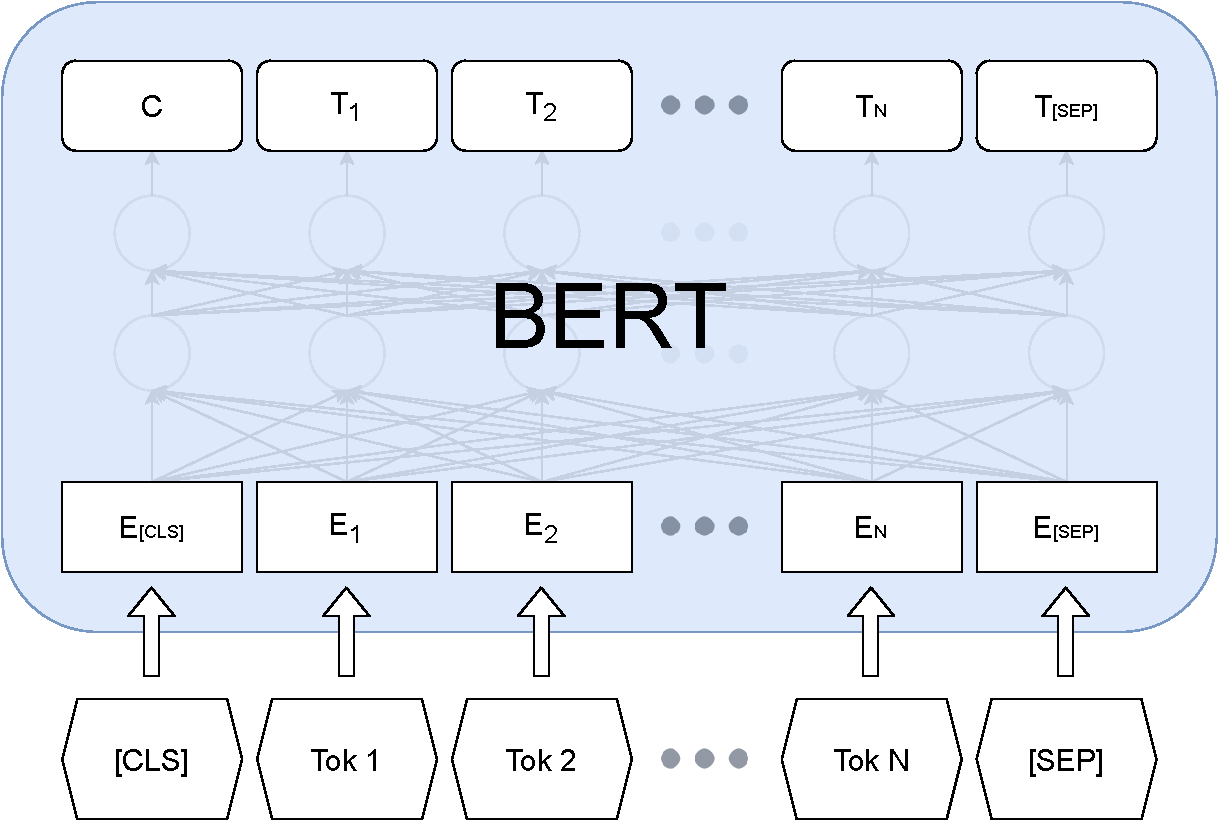
\includegraphics[width=\linewidth]{src/BERT.pdf}
	\caption{Schematic illustration of BERTs architecture.\newline
	Here the inputs and outputs that bert expects and delivers can be seen. Below the blue highlighted area we see the already tokenized words enclosed by the CLS and SEP token. These are now processed by BERT and one receives for each token the representation created by BERT visible here in the uppermost line. In between are representations that BERT uses as a kind of intermediate result. \newline
	Source: Adapted from \cite{Devlin2018}}
	\label{fig:bert}
\end{figure}
BERT is a modern approach to create a model that can take into account the context of a word in both directions. Thus, the model would be better able to interpret words through their context. Based on this architecture, a model is then pretrained on a corpus using masklm and nextsentence tasks. This base model can then be used for new tasks with relatively little effort. Tokens denote a representation for individual words that the model knows. These tokens can already be seen in the figure \ref{fig:bert}.

The masklm task consists of masking random words in a sentence and having the model guess what the masked word actually was. This task is commonly referred to as masked ML task or MLM for short. For training the original BERT model, about 15\% of all input tokens are masked and by predicting the missing words, BERT is supposed to learn an understanding of natural language. In the figure \ref{fig:bert} this would lead to the situation that some tokens of the lowest row are masked. \cite{Devlin2018}

The Next Sentence Prediction task consists of inferring relationships between two sentences. Because this task is not covered by MLM. The Next Sentence Prediction, or NSP for short, is intended to teach the model of a given sentence following a previously given one by means of a binary classification task. This task uses the CLS token as representation of the tokens that are to be classified. Especially QA and NLI are supposed to benefit from this training. \cite{Devlin2018}

These two tasks were then used to train BERT on the BooksCorpus and on English Wikipedia texts. At this point, a pretrained model is obtained, which can then be used in various ways depending on the particular task. Further training on a a new task is referred to as finetuning. \cite{Devlin2018}

Since finetuning tasks are quite specific, the details depend on the selected task. However, in general, the procedure can be classified into one of two groups. First, there are classification tasks based on complete sentences. These generally use the representation of the CLS token with a classifier layer. The other group of tasks operates at the token level and therefore uses the representation of the tokens using one or more additional layers. Both types of tokens can be seen in the figure \ref{fig:bert}.  Once the architecture is set, the fine-tuning can take place. This is done end to end, so the whole transformer, i.e. BERT and the task specific part are tuned together. If BERT is not supposed to be changed, there is generally the possibility to freeze specific layers and thus prevent the change of weights in these. This leads to the fact that for example only the task specific part of the transformer is trained. 

%\begin{itemize}
%	\item BERT as revolution
%	\item pretrained-models
%	\item usefull even without finetuning
%	\item $\Rightarrow$ unexpected precision
%	\item nowadays used for many different NLP tasks
%	\item Architecture of BERT
%	\begin{itemize}
%		\item explain corpora
%		\item explain vocabulary
%		\item explain tokenizer
%	\end{itemize}
%	\item extensions of BERT like roBERTa
%\end{itemize}

\section{BioBERT}
BioBERT can be viewed as an extension of BERT that emerged because BERT alone was not yielding the desired results in the biomedical domain. This observation has often been associated with the differences in word distributions between a general domain such as Wikipedia, on which BERT had been trained, and the highly specialized words that are frequently used or used only in the corresponding domain.\cite{Devlin2018,Lee2019,Liu2021} This difference in the underlying corpora not only implies that adaptations in the architecture of the model itself might be necessary, but moreover implies a possible need for adaptations in the vocabulary and tokenizer being used. \cite{Lee2019} 
\newline
Based on the knowledge that the vocabulary may differ significantly, it was hypothesized that a model that takes these features into account should perform significantly better on tasks within that specific domain than models that are more general and may not even have seen that domain previously. Based on this hypothesis, BioBERT was created. A model that is supposed to be better adapted to the biomedical domain than BERT. \cite{Lee2019}
\newline
Nevertheless, BioBERT itself is just a further trained version of BERT. This means that the original BERT model was used as a base and further trained on either PubMed abstracts, PubMed Central full-text articles, or both. Therefore, the authors chose to retain the original BERT vocabulary in order to use the pre-trained version of BERT as a foundation. This had the advantage that the original model only needed to be further trained on the new corpus and the required training time could be reduced significant. % <- das hier fehlt noch 
For the tokenizer WordPiece was used to handle the problem with unknown words. It was also considered to create a new vocabulary, but this idea was discarded in order to preserve the previously mentioned advantage of being able to utilize the pre-trained BERT model to save resources. 
As a result, it was observed that BioBERT performed better than BERT in version 1.0 that was based on PubMed abstracts and the full text articles of PubMed Central biomedical landscape with very few exceptions. Although the actual measured improvements sometimes vary quite significantly, it can be safely concluded that even continued training of BERT on a biomedical corpus can lead to significant improvements on tasks based in this domain. \cite{Lee2019}

\section{S2ORC-BERT}
S2ORC, known as the Semantic Scholar Open Research Corpus, is a corpus that contains a large number of papers as well as metadata and the references associated with the papers. According to the authors, the full text portion of the corpus alone is the largest structured academic text corpus available in April 2020.\cite{Lo2019} This corpus is based on semantic scholar papers and thus comes from several different origins. Although the main part of the paper is the acquisition and processing of papers and the resulting construction of the S2ORC corpus, the authors also use that corpus to continue training BERT. This is relatively close to the basic idea and approach behind BioBERT as well, but in this case is even closer to the approach used for SciBERT. \cite{Beltagy2019,Lo2019}

We will take a closer look at SciBERT at a later point in time. S2ORC-BERT, as the model trained here is called, unlike BioBERT, is trained from scratch and is therefore not based on the pretrained BERT model. Some important features are that the loss is calculated by cross entropy and the optimizer is Adam. The learning rate as well as the number of epochs per task are derived from two predefined sets. Here the combination is chosen that gives the best result for the respective task according to the development set. Since the S2ORC-BERT is rather used for validation of the corpus and clearly less focused on a new architecture for BERT, many parameters are identical to those of other papers, in particular the values reported for SciBERT were used.\cite{Lo2019} It should be mentioned that the difference between this model, BERT and SciBERT is almost exclusively due to the underlying corpus and the associated vocabulary.  




\section{OAG-BERT}
	Another approach that not only seeks to better match the corpus on which BERT is trained to the corresponding domain, but also simultaneously attempts to teach the model a more extensive understanding of the texts. With this further goal, however, the training strategy underlying BERT also needs to be adapted, because as we saw earlier, BERT's pretraining is based only on the MLM task and a NSP task. Although these two tasks together ensure that we obtain a reliable initial model, the question remains open whether specific tasks can be solved better by more directed training in the pretraining phase or by embedding additional information. \cite{Devlin2018,Liu2021}
	
	Based on this, one could argue that a model with domain entity knowledge might perform better than a model that does not utilize such information. For example, \citeauthor{Liu2021} argue that specific institutes may have a focus on certain scientific areas and that this knowledge has the potential to support the model in assigning a paper to a research area.\cite{Liu2021} While one might generally assume that the actual text should also provide enough information to assign a paper to research areas, this knowledge could still turn out to improve model performance. 
	
	Compared to existing approaches, OAG-BERT now tries to incorporate so-called non-homogeneous knowledge from the Open Academic Graph into the model. Here, non-homogeneous knowledge refers to information about authors, fields of study, venues and affiliation. 
	To integrate this information into the model 3 crucial changes are made compared to BERT. \cite{Liu2021}
	
	The first adaptation is the heterogeneous entity type embedding. Here the token type embeddings are replaced by entity type embeddings, so that the different information types receive unique labels, through which it is possible to identify which input belongs to which group. \cite{Liu2021}
	
	The next adaptation is the Entity-aware 2D-positional encoding. Just like BERT, OAG-BERT needs positional embeddings to encode the sequence order. However, BERT does not have the ability to distinguish between two adjacent entities and would interpret them as a single one. To solve this problem, the positional embeddings in OAG-BERT are two-dimensional and encode the so-called inter-entity sequence in the first dimension and the intra-entity sequence in the second dimension. \cite{Devlin2018,Liu2021}
	
	The last change is the span-aware entity masking. Although the masking strategy is not changed for the abstract or the actual text, a special masking is proposed for the new entity types. This is supposed to help OAG-BERT to learn complex entities especially if they consist of many tokens. So an entity consisting of four or less tokens will be completely masked, but as soon as it is longer only a part of the entity will be masked. The length of the mask is thereby drawn from a geometrical distribution.   
	The training can be grouped in two parts, the first part is only trained with normal texts. That means only abstract, main text and the title is used. The model obtained after this training is referred to by the authors as vanilla OAG-BERT. This is in contrast to the full OAG-BERT model. To obtain this, the vanilla model was now further trained using the heterogeneous entity information. \cite{Liu2021}
	
	In comparison with, for example, SciBERT, which was chosen by the authors for comparison, OAG-BERT performs very well in tasks involving the entities that are included under the term heterogeneous entities. However, it also shows that the gap between the two models can be greatly reduced by finetuning the entire SciBERT model. Thus, after finetuning, OAG-BERT can only significantly outperform in Venue and Affiliation and performs about as well as SciBERT in the field of study category.\cite{Liu2021}
%\section{Datasets}
%\begin{itemize}
%	\item zum Beispiel NCBI-Disease (versuch einen goldstandard für corpora zu erstellen)
%	\item sehr günstig um darauf entsprechende modelle zu trainieren \cite{Dogan2014}
%	\item SciERC /sciie im repo \cite{luan2018multitask}
%\end{itemize}
%\color{black}
%Due to the availability of the Datasets used by the original authors, we will use their prepared datasets, which are already prepared in a way that it is easier to use them for training and still only vary slightly from the original datasets. The datasets which we will use are directly retrieved from the SciBERT GitHub page and made available through the DataDeps package which provides an easy way to retrieve data that may or may not be locally available. If it is not already stored locally, it will be cached in the local Julia path and inside Julia, DataDeps provides the corresponding paths to the data and retrieves it from the defined source if needed. Furthermore, a hash can be defined as well to ensure that the provided data is identical to the expected one.\cite{White2019}\\
%In the following paragraph, we will take a closer look at the original data and the individual changes that have been made to use those Datasets for the training process.
%\subsection{Chemprot}
%Chemprot is in a JSON lines file format provided. More precisely every line consists of a text and the corresponding label. A field for metadata exists as well but is most of the time not used. In its original format, the Chemprot corpus consists of a develop, test, and train set of which the develop, test, and train folder correspond to the identically named files inside the chemprot folder provided on the GitHub site of SciBERT. The difference arises from a database-like structure in which the Chemprot corpus is originally provided, in contrast to those subdivided information sets where for example the text itself is in another file than the positions and annotations. Those divided pieces of information were combined and are provided in a single file in the already mentioned format. \cite{Beltagy2019,Wang2016}